\documentclass[11pt,a4paper]{article}
\usepackage{gtu-el-yazisi}
\begin{document}
\notbilgi{İşaretler ve Sistemler}{Ders 11 -- Ayrık Zamanlı Fourier Dönüşümü (DTFT)}{Isaret-ve-Sistemler-ders-11.pdf}

\section{Ayrık Zamanlı Fourier Transformu (Dönüşümü)}
\sayfa{1}
(Discrete-time Fourier Transform)

FT, periyodik olmayan işaretler için tanımlıdır.
\begin{align*}
  X(e^{j\omega})&=\sum_{n=-\infty}^{\infty}x[n]\,e^{-j\omega n}\\
  x[n]&=\frac{1}{2\pi}\int_{2\pi}X(e^{j\omega})\,e^{j\omega n}\,d\omega
\end{align*}
\begin{center}
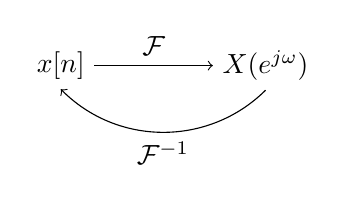
\begin{tikzpicture}
  \node (a) at (0,0) {$x[n]$};
  \node (b) at (2.6,0) {$X(e^{j\omega})$};
  \draw[->] (a) -- node[above] {$\mathcal{F}$} (b);
  \draw[->] (b.south) to[bend left=45] node[below] {$\mathcal{F}^{-1}$} (a.south);
\end{tikzpicture}
\end{center}
$\Rightarrow$ Ayrık zamanlı FT, $X(e^{j\omega})$ $2\pi$ ile periyodiktir.
\[ X(e^{j\omega})=X\bigl(e^{j(\omega+2\pi)}\bigr) \]

\begin{ornek}[]
  $x[n]=a^nu[n]$, \ $|a|<1$ ise $X(e^{j\omega})=\,?$
\end{ornek}
\[
  X(e^{j\omega})=\sum_{n=-\infty}^{\infty}x[n]e^{-j\omega n}
  \underset{\substack{\uparrow\\ u[n]=1,\ n\geq0}}{=}
  \sum_{n=0}^{\infty}a^ne^{-j\omega n}=\sum_{n=0}\bigl(ae^{-j\omega}\bigr)^n
  \underset{\substack{\uparrow\\ \sum_{k=0}^{\infty}\alpha^k=\frac{1}{1-\alpha},\ |\alpha|<1}}{=}
  \frac{1}{1-ae^{-j\omega}}
\]
\[ a^nu[n]\ \overset{\mathcal{F}}{\longleftrightarrow}\ \frac{1}{1-ae^{-j\omega}} \]
\begin{align*}
  X(e^{j\omega})&=|X(e^{j\omega})|\,e^{j\measuredangle X(e^{j\omega})}\\
  X(e^{j\omega})&=\frac{1}{1-ae^{-j\omega}}
  \underset{\substack{\uparrow\\ e^{-j\omega}=\cos\omega-j\sin\omega}}{=}
  \frac{1}{1-a\cos\omega+ja\sin\omega}\\
  |X(e^{j\omega})|&=\frac{1}{\sqrt{(1-a\cos\omega)^2+a^2\sin^2\omega}}=\frac{1}{\sqrt{1+a^2-2a\cos\omega}}\\
  \measuredangle X(e^{j\omega})&=-\operatorname{atan}\Bigl(\frac{a\sin\omega}{1-a\cos\omega}\Bigr)
\end{align*}
\begin{center}
\begin{tikzpicture}[xscale=0.42, yscale=0.9]
  \draw[->] (-8.6,0) -- (8.8,0) node[right] {$\omega$};
  \draw[->] (0,-0.2) -- (0,2.8) node[above] {$|X(e^{j\omega})|$};
  \draw[murekkep, thick, smooth] plot[domain=-8:8, samples=161] (\x, {1/sqrt(1.25-cos(deg(\x)))});
  \draw[dashed, kursunkalem] (-6.283,2) -- (6.283,2);
  \draw[dashed, kursunkalem] (-3.1416,0.667) -- (3.1416,0.667);
  \node[above right] at (0,2) {\scriptsize$1/(1-a)$};
  \node[above right] at (0,0.62) {\scriptsize$1/(1+a)$};
  \foreach \p/\l in {-6.283/-2\pi, -3.1416/-\pi, 3.1416/\pi, 6.283/2\pi}
    \draw (\p,0.06) -- (\p,-0.06) node[below] {\scriptsize$\l$};
  \node at (-9.2,1.5) {$\cdots$};
  \node at (9.2,1.5) {$\cdots$};
\end{tikzpicture}
\end{center}

\sayfa{2}
\begin{ornek}[]
  $x[n]=a^{|n|}$, \ $|a|<1$ ise $X(e^{j\omega})=\,?$
\end{ornek}
\[
  X(e^{j\omega})=\sum_{n=-\infty}^{\infty}x[n]e^{-j\omega n}=\sum_{n=-\infty}^{\infty}a^{|n|}e^{-j\omega n}
  =\sum_{n=-\infty}^{-1}a^{-n}e^{{\color{turuncukalem}-}j\omega n}+\sum_{n=0}^{\infty}a^{n}e^{-j\omega n}
\]
\[
  \sum_{n=-\infty}^{-1}\bigl(ae^{j\omega}\bigr)^{-n}
  \underset{\substack{\uparrow\\ k=-n}}{=}\sum_{k=1}^{\infty}{\color{turuncukalem}\bigl(}ae^{j\omega}{\color{turuncukalem}\bigr)}^k
  \underset{\substack{\uparrow\\ (ae^{j\omega})^0=1}}{=}\sum_{k=0}^{\infty}\bigl(ae^{j\omega}\bigr)^k-1
  =\frac{1}{1-ae^{+j\omega}}-1=\frac{ae^{j\omega}}{1-ae^{j\omega}}
\]
\[
  X(e^{j\omega})=\frac{ae^{j\omega}}{1-ae^{j\omega}}+\frac{1}{1-ae^{-j\omega}}=\frac{1-a^2}{1+a^2-2a\cos\omega}
  \ :\ \text{Reel}\qquad
  \begin{array}{l}
    X(e^{j\omega})=|X(e^{j\omega})|\\
    \measuredangle X(e^{j\omega})=0
  \end{array}
\]
\begin{center}
  \begin{tikzpicture}[scale=0.55]
    \draw[->] (-5.2,0) -- (5.4,0) node[right] {$n$};
    \draw[->] (0,-0.2) -- (0,3.4) node[above] {$x[n]$};
    \foreach \k in {-4,...,4} {
      \pgfmathsetmacro{\h}{2.6*0.72^(abs(\k))}
      \draw[murekkep, thick] (\k,0) -- (\k,\h); \fill[murekkep] (\k,\h) circle (3pt);}
    \node[left] at (0,2.75) {\scriptsize$1$};
    \node[right] at (1,1.87) {\scriptsize$a$};
    \node[right] at (2,1.35) {\scriptsize$a^2$};
    \node[right] at (3,0.97) {\scriptsize$a^3$};
    \node at (-5.4,0.6) {$\cdots$};
    \node at (4.9,0.6) {$\cdots$};
  \end{tikzpicture}\hspace{1cm}
  \begin{tikzpicture}[xscale=0.42, yscale=0.55]
    \draw[->] (-8.6,0) -- (8.8,0) node[right] {$\omega$};
    \draw[->] (0,-0.2) -- (0,5) node[above] {$|X(e^{j\omega})|$};
    \draw[murekkep, thick, smooth] plot[domain=-8:8, samples=241] (\x, {(1-0.36)/(1+0.36-1.2*cos(deg(\x)))});
    \draw[dashed, kursunkalem] (-6.283,4) -- (6.283,4);
    \node[above right] at (0,3.9) {\scriptsize$\frac{1-a}{1+a}$};
    \draw[dashed, kursunkalem] (-3.1416,0.25) -- (3.1416,0.25);
    \node[above left] at (0,0.25) {\scriptsize$\frac{1+a}{1-a}$};
    \foreach \p/\l in {-6.283/-2\pi, -3.1416/-\pi, 3.1416/\pi, 6.283/2\pi}
      \draw (\p,0.1) -- (\p,-0.1) node[below] {\scriptsize$\l$};
  \end{tikzpicture}\footnote{Claude notu: etiketler yer değiştirmiş görünüyor; muhtemelen tepe değeri ($\omega=0$) $\frac{1+a}{1-a}$, en küçük değer ($\omega=\pm\pi$) $\frac{1-a}{1+a}$ olmalı.}
\end{center}
\[
  a^{|n|}\ \overset{\mathcal{F}}{\longleftrightarrow}\ \frac{1-a^2}{1+a^2-2a\cos\omega}
\]

\begin{ornek}[]
  $x[n]=\begin{cases}1, & |n|\leq N_1\\ 0, & |n|>N_1\end{cases}$ \ şeklinde verilen ayrık zamanlı dikdörtgen darbe işaretinin FT bulunuz.
\end{ornek}
\begin{align*}
  X(e^{j\omega})&=\sum_{n=-\infty}^{\infty}x[n]e^{-j\omega n}=\sum_{n=-N_1}^{N_1}e^{-j\omega n}
    =\sum_{n=0}^{2N_1}e^{-j\omega(n-N_1)}=e^{j\omega N_1}\sum_{n=0}^{2N_1}e^{-j\omega n}\\
  &=e^{j\omega N_1}\left[\frac{1-e^{-j\omega(2N_1+1)}}{1-e^{-j\omega}}\right]\\
  &=e^{j\omega N_1}\,\frac{e^{-j\omega(N_1+1/2)}\bigl[e^{j\omega(N_1+1/2)}-e^{-j\omega(N_1+1/2)}\bigr]}{e^{-j\omega/2}\bigl[e^{j\omega/2}-e^{-j\omega/2}\bigr]}\\
  &=\frac{\sin\bigl(\omega(N_1+1/2)\bigr)}{\sin(\omega/2)}
\end{align*}
Reminder: \quad $\displaystyle\sum_{k=0}^{M}\alpha^k=\frac{1-\alpha^{M+1}}{1-\alpha}$,
\qquad $1-e^{j\theta}=e^{-j\theta/2}\bigl[e^{j\theta/2}-e^{-j\theta/2}\bigr]$\footnote{Claude notu: sağ taraf $1-e^{-j\theta}$'ya eşittir; muhtemelen sol taraf $1-e^{-j\theta}$ olmalı.}

\medskip
$N_1=2$ için
\begin{center}
  \begin{tikzpicture}[scale=0.55]
    \draw[->] (-5,0) -- (5,0) node[right] {$n$};
    \draw[->] (0,-0.2) -- (0,2.6) node[above] {$x[n]$};
    \foreach \k in {-2,...,2} {\draw[murekkep, thick] (\k,0) -- (\k,1.6); \fill[murekkep] (\k,1.6) circle (3pt);}
    \foreach \k in {-4,-3,3,4} \fill[murekkep] (\k,0) circle (3pt);
    \node[above left] at (0,1.6) {\scriptsize$1$};
    \node[below, turuncukalem] at (-2,0) {\scriptsize$-N_1$};
    \node[below, turuncukalem] at (2,0) {\scriptsize$N_1$};
  \end{tikzpicture}\hspace{0.8cm}
  \begin{tikzpicture}[xscale=0.45, yscale=0.42]
    \draw[->] (-7.6,0) -- (7.9,0) node[right] {$\omega$};
    \draw[->] (0,-2) -- (0,6.2) node[above] {$X(e^{j\omega})$};
    \draw[murekkep, thick, smooth] plot[domain=-7.2:7.2, samples=200] (\x, {sin(deg(2.5*\x))/sin(deg(\x/2))});
    \node[above right] at (0,5) {\scriptsize$5$};
    \foreach \p/\l in {-6.283/-2\pi, -3.1416/-\pi, 3.1416/\pi, 6.283/2\pi}
      \draw (\p,0.12) -- (\p,-0.12) node[below] {\scriptsize$\l$};
  \end{tikzpicture}
\end{center}

\sayfa{3}
\providecommand{\ciz}[1]{\tikz[baseline=(c.base)]{\node[inner sep=0pt] (c) {$#1$}; \draw[turuncukalem, thick] (c.south west) -- (c.north east);}}
\begin{ornek}[]
  $x[n]=\delta[n]$
\end{ornek}
\[
  X(e^{j\omega})=\sum_{n=-\infty}^{\infty}x[n]e^{-j\omega n}=\sum_{n=-\infty}^{\infty}\delta[n]e^{-j\omega n}
  \underset{\substack{\uparrow\\ \delta[n]=1,\ n=0}}{=}e^{-j\omega0}=1
\]

\begin{ornek}[]
  $X(e^{j\omega})=\delta(e^{j\omega})$ ise $x[n]=\,?$
\end{ornek}
\[
  x[n]=\frac{1}{2\pi}\int_{2\pi}X(e^{j\omega})e^{j\omega n}\,d\omega
  =\frac{1}{2\pi}\int_{-\pi}^{\pi}\delta(e^{j\omega})e^{j\omega n}\,d\omega
  =\frac{1}{2\pi}\int_{-\pi}^{\pi}\delta(e^{j\omega})\underbrace{e^{j0n}}_{1}\,d\omega=\frac{1}{2\pi}
\]
\begin{center}
  \begin{tikzpicture}[xscale=0.5, yscale=0.8]
    \draw[->] (-8.2,0) -- (8.4,0) node[right] {$\omega$};
    \draw[->] (0,-0.2) -- (0,2.2) node[above] {$X(e^{j\omega})$};
    \foreach \p in {-6.283,0,6.283} \draw[->, murekkep, thick] (\p,0) -- (\p,1.4);
    \node[right] at (0,1.4) {\scriptsize$1$};
    \foreach \p/\l in {-6.283/-2\pi, -3.1416/-\pi, 3.1416/+\pi, 6.283/2\pi}
      \draw (\p,0.08) -- (\p,-0.08) node[below] {\scriptsize$\l$};
    \node at (-8,0.8) {$\cdots$};
    \node at (8,0.8) {$\cdots$};
  \end{tikzpicture}
\end{center}
\begin{align*}
  \delta[n]&\ \overset{\mathcal{F}}{\longleftrightarrow}\ 1\\
  1&\ \longleftrightarrow\ 2\pi\,\delta(e^{j\omega})
\end{align*}

\begin{ornek}[]
  $x[n]=\delta[n-n_0]$
\end{ornek}
\[
  X(e^{j\omega})=\sum_{n=-\infty}^{\infty}x[n]e^{-j\omega n}=\sum_{n=-\infty}^{\infty}\delta[n-n_0]e^{-j\omega n}
  \underset{\substack{\uparrow\\ \delta[n-n_0]=1,\ n=n_0}}{=}e^{-j\omega n_0}
\]
\[ \delta[n-n_0]\ \longleftrightarrow\ e^{-j\omega n_0} \]

\begin{ornek}[]
  $X(e^{j\omega})=\delta\bigl(e^{j(\omega-\omega_0)}\bigr)$ ise $x[n]=\,?$
\end{ornek}
\begin{align*}
  x[n]&=\frac{1}{2\pi}\int_{2\pi}X(e^{j\omega})e^{j\omega n}\,d\omega
    =\frac{1}{2\pi}\int_{-\pi}^{\pi}\delta\bigl(e^{j(\omega-\omega_0)}\bigr)e^{j\omega n}\,d\omega\\
  &=\frac{1}{2\pi}\int_{2\pi}\delta\bigl(e^{j(\omega-\omega_0)}\bigr)e^{j\omega_0n}\,d\omega\\
  &=\frac{1}{2\pi}e^{j\omega_0n}\underbrace{\int_{-\pi}^{\pi}\delta\bigl(e^{j(\omega-\omega_0)}\bigr)\,d\omega}_{=1}
    =\frac{1}{\ciz{2\pi}}e^{j\omega_0n}
\end{align*}
\begin{align*}
  e^{j\omega_0n}&\ \overset{\mathcal{F}}{\longleftrightarrow}\ 2\pi\,\delta\bigl(e^{j(\omega-\omega_0)}\bigr)\\
  e^{-j\omega_0n}&\ \overset{\mathcal{F}}{\longleftrightarrow}\ 2\pi\,\delta\bigl(e^{j(\omega+\omega_0)}\bigr)
\end{align*}

\section{Periyodik işaretlerin Fourier Transformu}
\sayfa{4}
\[
  x[n]=x[n+N],\ \ \forall n,\qquad N=\frac{2\pi}{\omega_0},\qquad \omega_0=\frac{2\pi}{N}
\]
\[
  x[n]=\sum_{k=\langle N\rangle}x_ke^{jk\omega_0n}=x_0+x_1e^{j\omega_0n}+x_2e^{j2\omega_0n}+\cdots+x_{N-1}e^{j(N-1)\omega_0n}
\]
\[
  x_k=\frac{1}{N}\sum_{n=\langle N\rangle}x[n]e^{-jk\omega_0n},\qquad x_k=x_{k+N}\ \longleftarrow\
  \begin{array}{l} x_0=x_N\\ x_1=x_{N+1}\\ \ \ \vdots\end{array}
\]
\[ x[n]=\sum_{k=\langle N\rangle}x_ke^{jk\omega_0n}\ \overset{\mathcal{F}}{\longleftrightarrow}\ X(e^{j\omega})=\sum_{k=-\infty}^{\infty}2\pi x_k\,\delta(\omega-k\omega_0) \]

\begin{ornek}[]
  $x[n]=\cos\bigl(\frac{2\pi n}{5}\bigr)$ ise $X(e^{j\omega})=\,?$
\end{ornek}
\[
  x[n]=\frac12e^{j(2\pi n/5)}+\frac12e^{-j(2\pi n/5)},\qquad
  \begin{array}{l}\omega_0=2\pi/5\\ x_1=x_{-1}=1/2\end{array}
\]
\[ \Big\updownarrow\,\mathcal{F} \]
\[
  X(e^{j\omega})=\pi\,\delta(\omega-2\pi/5)+\pi\,\delta(\omega+2\pi/5),\qquad -\pi\leq\omega<\pi
\]
\begin{center}
  \begin{tikzpicture}[xscale=0.62, yscale=0.8]
    \draw[->] (-8.8,0) -- (9.2,0) node[right] {$\omega$};
    \draw[->] (0,-0.2) -- (0,2.4) node[above] {$X(e^{j\omega})$};
    \foreach \p in {-7.5,-5,-1.25,1.25,5,7.5} \draw[->, murekkep, thick] (\p,0) -- (\p,1.4);
    \draw (-0.08,1.4) -- (0.08,1.4) node[above right] {\scriptsize$\pi$};
    \draw[dashed, kursunkalem] (-8.3,1.4) -- (8.3,1.4);
    \draw (-6.25,0.08) -- (-6.25,-0.08); \draw (6.25,0.08) -- (6.25,-0.08);
    \node[below] at (-7.6,0) {\tiny$-2\pi-\omega_0$};
    \node[below] at (-6.25,-0.35) {\tiny$-2\pi$};
    \node[below] at (-4.9,0) {\tiny$-2\pi+\omega_0$};
    \node[below] at (-1.25,0) {\tiny$-\omega_0$};
    \node[below] at (1.25,0) {\tiny$\omega_0$};
    \node[below] at (4.9,0) {\tiny$2\pi-\omega_0$};
    \node[below] at (6.25,-0.35) {\tiny$2\pi$};
    \node[below] at (7.6,0) {\tiny$2\pi+\omega_0$};
    \node at (-9.2,0.8) {$\cdots$};
    \node at (8.6,1.0) {$\cdots$};
  \end{tikzpicture}
\end{center}

\begin{ornek}[]
  $x[n]=\displaystyle\sum_{k=-\infty}^{\infty}\delta[n-kN]$ \ periyodik dürtü treninin FT bulunuz.
\end{ornek}
Reminder: \quad $x_k=\dfrac1N\displaystyle\sum_{n=\langle N\rangle}x[n]e^{-jk\omega_0n}=\dfrac1N$
\[
  X(e^{j\omega})=\frac{2\pi}{N}\sum_{k=-\infty}^{\infty}\delta\Bigl(\omega-\frac{2\pi k}{N}\Bigr)
\]
\begin{center}
  \begin{tikzpicture}[scale=0.5]
    \draw[->] (-5.6,0) -- (5.8,0) node[right] {$n$};
    \draw[->] (0,-0.2) -- (0,2.6) node[above] {$x[n]$};
    \foreach \k in {-4,-2,0,2,4} {\draw[murekkep, thick] (\k,0) -- (\k,1.6); \fill[murekkep] (\k,1.6) circle (3pt);}
    \draw[turuncukalem, very thick] (-0.6,0) -- (-0.6,1.4);
    \draw[turuncukalem, very thick] (0.6,0) -- (0.6,1.4);
    \node[above right] at (0,1.6) {\scriptsize$1$};
    \foreach \k/\l in {-4/-2N,-2/-N,0/0,2/N,4/2N} \node[below] at (\k,0) {\scriptsize$\l$};
    \node at (-5.4,0.8) {$\cdots$};
    \node at (5.3,0.8) {$\cdots$};
  \end{tikzpicture}\hspace{1.2cm}
  \begin{tikzpicture}[scale=0.5]
    \draw[->] (-5.6,0) -- (5.8,0) node[right] {$\omega$};
    \draw[->] (0,-0.2) -- (0,2.8) node[above] {$X(e^{j\omega})$};
    \foreach \k in {-4,-2,0,2,4} \draw[->, murekkep, thick] (\k,0) -- (\k,1.6);
    \node[right] at (0,1.9) {\scriptsize$\frac{2\pi}{N}$};
    \foreach \k/\l in {-2/-\frac{2\pi}{N},0/0,2/\frac{2\pi}{N}} \node[below] at (\k,0) {\scriptsize$\l$};
    \node at (-5.4,0.8) {$\cdots$};
    \node at (5.3,0.8) {$\cdots$};
  \end{tikzpicture}
\end{center}

\section{Ayrık Zamanlı Fourier Transformunun Özellikleri}
\sayfa{5}
\begin{align*}
  &x[n]\ \overset{\mathcal{F}}{\longleftrightarrow}\ X(e^{j\omega})\\
  &X(e^{j\omega})=\mathcal{F}\{x[n]\}\\
  &x[n]=\mathcal{F}^{-1}\{X(e^{j\omega})\}
\end{align*}
\begin{enumerate}[label=\arabic*)]
  \item \textbf{Periyodiklik:} \ $X(e^{j\omega})=X\bigl(e^{j(\omega+2\pi)}\bigr)$, \ $2\pi$ ile periyodiktir.
  \item \textbf{Lineerlik:} \ $\alpha x_1[n]+\beta x_2[n]\ \overset{\mathcal{F}}{\longleftrightarrow}\ \alpha X_1(e^{j\omega})+\beta X_2(e^{j\omega})$
  \item \textbf{Zamanda öteleme:} \ $x[n-n_0]\ \overset{\mathcal{F}}{\longleftrightarrow}\ e^{-j\omega n_0}X(e^{j\omega})$\\
    Genlik spektrumu değişmez, faz spektrumu $-\omega n_0$ kadar ötelenir.
  \item \textbf{Frekansta öteleme:} \ $e^{j\omega_0n}x[n]\ \overset{\mathcal{F}}{\longleftrightarrow}\ X\bigl(e^{j(\omega-\omega_0)}\bigr)$
  \item \textbf{Zamanda katlama:} \ $x[-n]\ \overset{\mathcal{F}}{\longleftrightarrow}\ X(e^{-j\omega})$
  \item \textbf{Eşlenik alma:} \ $x^*[n]\ \overset{\mathcal{F}}{\longleftrightarrow}\ X^*(e^{-j\omega})$
  \item \textbf{Fark alma (differencing):} \ $x[n]-x[n-1]\ \overset{\mathcal{F}}{\longleftrightarrow}\ (1-e^{-j\omega})X(e^{j\omega})$
  \item \textbf{Birikim (Accumulation):}
    \[ \sum_{m=-\infty}^{n}x[m]\ \overset{\mathcal{F}}{\longleftrightarrow}\ \frac{1}{1-e^{-j\omega}}X(e^{j\omega})+\pi X(e^{j0})\sum_{k=-\infty}^{\infty}\delta(\omega-2\pi k) \]
  \item \textbf{Frekansta türev:} \ $n\,x[n]\ \overset{\mathcal{F}}{\longleftrightarrow}\ j\,\dfrac{dX(e^{j\omega})}{d\omega}$\par
    İspat: \ $X(e^{j\omega})=\displaystyle\sum_{n=-\infty}^{\infty}x[n]e^{-j\omega n}$
    \[ \frac{d}{d\omega}X(e^{j\omega})=\sum_{n=-\infty}^{\infty}x[n]\frac{d}{d\omega}\bigl(e^{-j\omega n}\bigr)=-jn\sum_{n=-\infty}^{\infty}x[n]e^{-j\omega n}\text{\footnotemark} \]
    \footnotetext{Claude notu: $n$ toplam indisidir, toplamın dışına çıkamaz; muhtemelen $=-j\sum_{n} n\,x[n]e^{-j\omega n}$ olmalı.}
  \item \textbf{Parseval teoremi:} \ $E_x=\displaystyle\sum_{n=-\infty}^{\infty}|x[n]|^2=\frac{1}{2\pi}\int_{2\pi}|X(e^{j\omega})|^2\,d\omega$
  \item \textbf{Çarpma:} \ $x_1[n]\cdot x_2[n]\ \overset{\mathcal{F}}{\longleftrightarrow}\ \dfrac{1}{2\pi}\displaystyle\int_{2\pi}X_1(e^{j\alpha})X_2\bigl(e^{j(\omega-\alpha)}\bigr)\,d\alpha$
  \item \textbf{Konvolüsyon:} \ $x_1[n]*x_2[n]\ \overset{\mathcal{F}}{\longleftrightarrow}\ X_1(e^{j\omega})X_2(e^{j\omega})$
    \begin{center}
      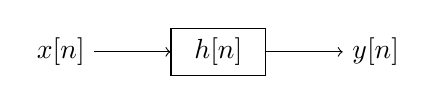
\begin{tikzpicture}
        \node (x) at (0,0) {$x[n]$};
        \node[draw, rectangle, minimum width=1.2cm, minimum height=0.6cm] (h) at (2,0) {$h[n]$};
        \node (y) at (4,0) {$y[n]$};
        \draw[->] (x) -- (h); \draw[->] (h) -- (y);
      \end{tikzpicture}
    \end{center}
    \[
      y[n]=x[n]*\underset{\substack{\downarrow\\ \text{Dürtü cevabı}}}{h[n]}
      \ \overset{\mathcal{F}}{\longleftrightarrow}\
      Y(e^{j\omega})=X(e^{j\omega})\underset{\substack{\downarrow\\ \text{Frekans cevabı}}}{H(e^{j\omega})}
    \]
    \[
      H(e^{j\omega})=\frac{Y(e^{j\omega})}{X(e^{j\omega})}\ \overset{\mathcal{F}^{-1}}{\longleftrightarrow}\ h[n]
    \]
\end{enumerate}

\sayfa{6}
\begin{ornek}[]
  $x[n]=u[n]$ ise $X(e^{j\omega})=\,?$
\end{ornek}
Reminder: \quad $u[n]=\displaystyle\sum_{k=-\infty}^{n}\delta[k]=\sum_{k=0}^{\infty}\delta[n-k]$
\begin{align*}
  \sum_{m=-\infty}^{n}x[m]\ &\overset{\mathcal{F}}{\longleftrightarrow}\ \frac{1}{1-e^{-j\omega}}X(e^{j\omega})+\pi X(e^{j0})\sum_{k=-\infty}^{\infty}\delta(\omega-2\pi k)\\
  \delta[n]\ &\overset{\mathcal{F}}{\longleftrightarrow}\ 1
\end{align*}
\[
  u[n]\ \overset{\mathcal{F}}{\longleftrightarrow}\ \frac{1}{1-e^{-j\omega}}+\pi\sum_{k=-\infty}^{\infty}\delta(\omega-2\pi k)
\]

\begin{ornek}[]
  $H(e^{j\omega})=\begin{cases}1, & 0\leq|\omega|\leq\omega_c\\ 0, & \omega_c<|\omega|<\pi\end{cases}$
  \quad ayrık zamanlı alçak geçiren filtrenin dürtü cevabını bulunuz.
\end{ornek}
\begin{center}
  \begin{tikzpicture}[xscale=0.55, yscale=0.9]
    \draw[->] (-8.6,0) -- (8.8,0) node[right] {$\omega$};
    \draw[->] (0,-0.2) -- (0,2) node[above] {$H(e^{j\omega})$};
    \foreach \c in {-6.283,0,6.283} \draw[murekkep, thick] (\c-1.1,0) -- (\c-1.1,1.2) -- (\c+1.1,1.2) -- (\c+1.1,0);
    \node[above right] at (0,1.2) {\scriptsize$1$};
    \foreach \p/\l in {-6.283/-2\pi, -3.1416/-\pi, -1.1/-\omega_c, 1.1/\omega_c, 3.1416/\pi, 6.283/2\pi}
      \draw (\p,0.08) -- (\p,-0.08) node[below] {\scriptsize$\l$};
    \node at (-8.4,0.8) {$\cdots$};
    \node at (8.4,0.8) {$\cdots$};
  \end{tikzpicture}
\end{center}
\begin{align*}
  h[n]&=\frac{1}{2\pi}\int_{2\pi}H(e^{j\omega})e^{+j\omega n}\,d\omega=\frac{1}{2\pi}\int_{-\omega_c}^{\omega_c}e^{j\omega n}\,d\omega
    =\frac{1}{2\pi}\,\frac{e^{j\omega n}}{jn}\bigg|_{-\omega_c}^{\omega_c}=\frac{1}{2j\pi n}\bigl[e^{j\omega_cn}-e^{-j\omega_cn}\bigr]\\
  h[n]&=\frac{1}{\pi n}\sin(\omega_cn)=\frac{\sin\bigl(\pi\frac{\omega_c}{\pi}n\bigr)}{\pi\frac{\omega_c}{\pi}n}\cdot\frac{\omega_c}{\pi}
    =\frac{\omega_c}{\pi}\,\mathrm{sinc}\Bigl(\frac{\omega_c}{\pi}n\Bigr)
\end{align*}
\begin{center}
  \begin{tikzpicture}[xscale=0.3, yscale=1]
    \draw[->] (-12.5,0) -- (13,0) node[right] {$n$};
    \draw[->] (0,-0.6) -- (0,2.2) node[above] {$h[n]$};
    \draw[dashed, kursunkalem, smooth] plot[domain=-11.5:11.5, samples=100] (\x, {1.6*sin(180*\x/7)/(pi*\x/7)});
    \foreach \k in {-11,...,11} {
      \ifnum\k=0 \pgfmathsetmacro{\h}{1.6}\else \pgfmathsetmacro{\h}{1.6*sin(180*\k/7)/(pi*\k/7)}\fi
      \draw[murekkep, thick] (\k,0) -- (\k,\h); \fill[murekkep] (\k,\h) circle (0.1 and 0.03);}
    \node at (-12.8,0.5) {$\cdots$};
    \node at (12.4,0.4) {$\cdots$};
  \end{tikzpicture}
\end{center}

\end{document}
